\section{Using \padx{} to Query Ad Hoc Data}
\label{section:padx}

\begin{figure}
\begin{center}
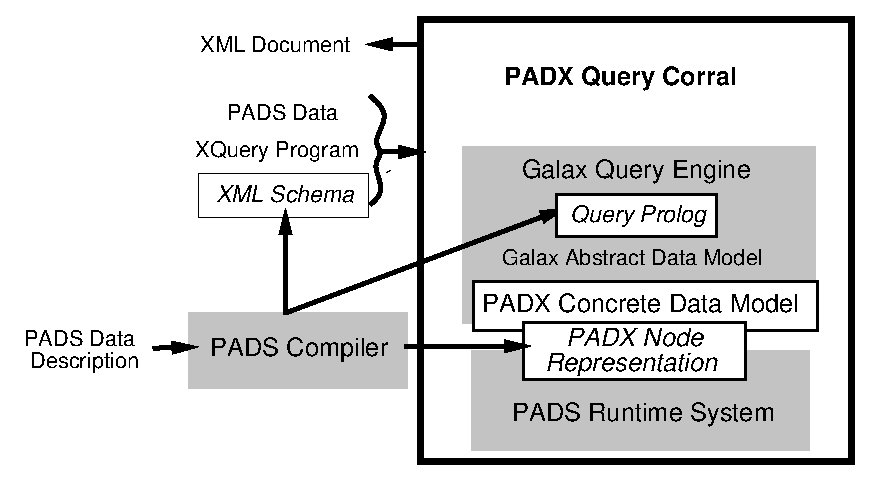
\epsfig{file=padx-arch.ps,width=0.47\textwidth}
\end{center}
\caption{Internal view of \padx{} Architecture}
\label{figure:padx-arch}
\end{figure}

Figure~\ref{figure:padx-arch} depicts an internal view of the \padx{}
architecture first shown in Figure~\ref{figure:padx-arch1}.
Pre-existing components (in grey boxes) include the \pads{} compiler,
the \Galax{} query engine, and the \pads{} runtime system.  In this
section, we focus on the new components (in white boxes) and describe
the compiler and run-time support for viewing \pads{} data as XML.
From a \pads{} description, the compiler generates an XML Schema
description that specifies the virtual XML view of the corresponding
\pads{} data; an XQuery prolog that imports the generated schema and
that associates the input data with the correct schema type; and a
type-specific library that provides the virtual XML view of \pads{}
values necessary to implement \padx{}'s concrete data model.  

Note that a query corral is \emph{customized} for a particular \pads{}
description, in particular, its concrete data model only supports
views of data sources that match the \pads{} description.  To maintain
the correct correspondence between a description, XML Schema, queries,
and data, the query corral explicitly contains the generated query
prolog, which imports the XML Schema that corresponds to the
underlying type-specific library.  This guarantees that the user's
XQuery program is statically typed, compiled, and optimized with
respect to the correct XML Schema and that the underlying data model
is an instance of this XML Schema.  At runtime, the query corral takes
an XQuery program and a \pads{} data source and produces the query
result in XML.  We discuss the problem of producing native \pads{}
values in Section~\ref{section:future}.

\subsection{Viewing \pads{} data as XML}	

The mapping from a \pads{} description to an XML Schema is 
straight-forward.  The interesting aspect of this mapping is that both
\pads{} values that are error free and those containing errors are
accessible in the XML view.  We begin with the mapping of \pads{} base
types. 

A default XML Schema, \cd{pads.xsd}, contains the schema types that
represent the \pads{} base types shared by all \pads{} descriptions.
Figure~\ref{figure:pads.xsd} contains a fragment of this schema.
Every \pads{} base type is mapped to the schema simple type that most
closely subsumes the value space of the given \pads{} base type.  For example,
the \cd{Puint32} base type maps to the schema type \cd{xs:unsignedInt}
(Lines~1--3).  Recall that all parsed \pads{} values have an in-memory
representation and a parse descriptor, which records the state of the
parse, the error code for detected errors, and the location of those
errors.  The XML view of a parsed value is a choice of the in-memory
representation (\cd{rep}), if no error occurred, or of the parse
descriptor (\cd{pd}), if
an error occurred (Lines~4--8).  This light-weight view exposes the
parse descriptor only when an error occurs.  The parse-descriptor type
for all base types is represented by the schema type
\cd{Pbase\_pd} (Line~10--14).

\begin{figure}
\begin{small}
\begin{code}
 1. <xs:simpleType name="\kw{base\_Puint32}">
 2.  <xs:restriction base="\kw{xs:unsignedInt}"/>
 3. </xs:simpleType>
 4. <xs:complexType name="\kw{val_Puint32}">
 5.  <xs:\kw{choice}>
 6.   <xs:element name="\kw{rep}" type="\kw{p:base\_Puint32}"/>
 7.   <xs:element name="\kw{pd}"  type="\kw{p:Pbase_pd}"/>
 8.  </xs:\kw{choice}>
 9. </xs:complexType>
{10}. <xs:complexType name="\kw{Pbase_pd}">
{11}.  <xs:sequence>
{12}.   <xs:element name="\kw{pstate}"  type="\kw{p:Pflags_t}"/>
{13}.   <xs:element name="\kw{errCode}" type="\kw{p:PerrCode_t}"/>
{14}.   <xs:element name="\kw{loc}"     type="\kw{p:Ploc_t}"/>
{15}.  </xs:sequence>
{16}. </xs:complexType>
\end{code}
\end{small}
\caption{Fragment of XML Schema for \pads{} base types.}
\label{figure:pads.xsd}
\end{figure}

The fragment of the XML Schema in Figure~\ref{figure:dibbler-schema}
corresponds to the description in Figure~\ref{figure:dibbler}.  Note
that the schema imports the schema for \pads{} base types (Line~5).
Each compound type is mapped to a complex schema type with a
particular content model.  A \kw{Pstruct} is mapped to a complex type
that contains a sequence of local elements, each of which corresponds
to one field in the \kw{Pstruct}.  For example, the \kw{Pstruct}
\cd{order\_header\_t} is mapped to the complex type
\cd{order\_header\_t} (Lines~7--15), which contains an element
declaration for the field \cd{order\_num}, among others.  A
\kw{Punion} is mapped to a complex type that contains a choice of
elements, each of which corresponds to one field in the \kw{Punion}.
\begin{figure*}
\begin{small}
\begin{code}
{ 1}. <xs:schema targetNamespace="\kw{file:/example/sirius.p}"
{ 2}.            xmlns="file:/example/sirius.p"
{ 3}.            xmlns:xs="http://www.w3.org/2001/XMLSchema"
{ 4}.            xmlns:p="http://www.padsproj.org/pads.xsd">
{ 5}. <xs:import namespace = "\kw{http://www.padsproj.org/pads.xsd}".../>
{ 6}. ...
{ 7}. <xs:complexType name="\kw{order_header_t}">
{ 8}.  <xs:sequence>
{ 9}.   <xs:element name="\kw{order_num}"     type="\kw{p:val_Puint32}"/>
{10}.   <xs:element name="\kw{att_order_num}" type="\kw{p:val_Puint32}"/>
{11}.   <xs:element name="\kw{ord_version}"   type="\kw{p:val_Puint32}"/>
{12}.   <!-- More local element declarations -->
{13}.   <xs:element name="\kw{pd}"            type="\kw{p:PStruct_pd}" minOccurs="0"/>
{14}.  </xs:sequence>
{15}. </xs:complexType>
{16}. <!-- More complex type declarations -->
{17}. <xs:complexType name="\kw{orders_t}">
{18}.  <xs:sequence>
{19}.   <xs:element name="\kw{elt}"    type="\kw{order_t}" maxOccurs="unbounded"/>
{20}.   <xs:element name="\kw{length}" type="\kw{p:Puint32}"/>
{21}.   <xs:element name="\kw{pd}"     type="\kw{p:Parray_pd}" minOccurs="0"/>
{22}.  </xs:sequence>
{23}. </xs:complexType>
     ...
{24}. <xs:element name="\kw{Psource}" type="\kw{summary_t}"/>
{25}. </xs:schema>
\end{code}
\end{small}
\caption{Fragment of XML Schema for \dibbler{} \pads{} description.}
\label{figure:dibbler-schema}
\end{figure*}

Each complex type also includes an optional \cd{pd} element that
corresponds to the type's parse descriptor (Lines~13 and~21).  All
parse-descriptor types contain the parse state, error code, and
location.  The parse-descriptor for compound types contain additional
information, \eg{}, \cd{Pstruct\_pd} contains the number of nested
errors and \cd{Parray\_pd} contains the index of the array item in
which the first error occurred.  The \cd{pd} element is absent if no
errors occurred during parsing, but if present, permits an analyst to
easily identify the kind and location of errors in the source data.
For example, the following XQuery expression returns the locations of all
orders that contain at least one error:
\cd{$pads/Psource/orders/elt/pd/loc}.

The schema types for some compound types contain additional fields
from the \pads{} in-memory representation, \eg{} arrays have a length
(Line~20).  Note that \cd{Parray} types do not associate a name with
each individual array item, so in the corresponding schema type, the
default element \cd{elt} encapsulates each array item.

The \pads{} compiler generates a query prolog that specifies the
environment in which all XQuery programs over the corresponding data
are typed and evaluated. 
Figure~\ref{figure:padx-query-prolog} contains the query prolog for
the schema in Figure~\ref{figure:dibbler-schema}.  The import schema
declaration on Line~1 imports the schema in
Figure~\ref{figure:dibbler-schema}.  This declaration puts all global
element and type declarations in scope for the query.  The variable
declaration on Line~2 specifies that the value of the variable
\cd{\$pads} is provided externally and that its type is a document
whose top-level element is of type \cd{Psource}, defined on Line~24 in
Figure~\ref{figure:dibbler-schema}.  This declarations guarantee
that the query is statically typed with respect to the correct input type.

At run time, the user can specify
the input data as a command-line argument or by calling the XQuery
\cd{fn:doc} function on a \pads{} source, \eg{} \cd{pads:/example/sirius.data}.
\begin{figure*}
\begin{small}
\begin{code}
 1. import schema default element namespace "\kw{file:/example/sirius.p}";
 2. declare variable \kw{$pads} as \kw{document-node(Psource)} external; 
\end{code}
\end{small}
\caption{\padx{} generated query prolog}
\label{figure:padx-query-prolog}
\end{figure*}

\subsection{\padx{} Concrete Data Model}

In Figure~\ref{figure:padx-arch}, the interface between \Galax{} and
\pads{} consists of two modules: the generic \padx{} concrete data model,
which implements the \Galax{} abstract data model, and a
compiler-generated module, in which each \pads{} type has a
corresponding, type-specific node representation providing the XML
view of values of that type.

Figure~\ref{fig:padx-element-node} contains a fragment of the \padx{}
concrete data model for a node.  This object provides a thin wrapper
around the type-specific node representation, \cd{padx\_node\_rep},
whose interface is in Figure~\ref{fig:padx-node-rep}.  A node
representation contains references to a \pads{} value's in-memory
representation and parse descriptor.  The node representation
interface returns the \Xml{} view of the \pads{} value, including the
value's element name, its typed value, and parent.
The \cd{kth\_child} and \cd{kth\_child\_by\_name} methods 
return all of the \pads{} value's children in order and those with a
given name in order, respectively.
\begin{figure*}
\begin{small}
\begin{code}
class virtual padx\_node\_rep :
  object 
    (* Private data includes parsed value's rep \& pd *)
    method name        : unit -> string
    method typed_value : unit -> item
    method parent      : unit -> padx\_node\_rep option
    method kth\_child   : int -> padx\_node\_rep option
    method kth\_child\_by\_name : int -> string -> padx\_node\_rep option
  end
\end{code}
\end{small}
\caption{The \padx{} node representation}
\label{fig:padx-node-rep}
\end{figure*}

For some methods in Figure~\ref{fig:padx-element-node} (Lines~4--5),
the concrete data model simply invokes the corresponding type-specific
methods.  One exception is the \cd{child} axis method (Lines~7--17),
which we describe in detail as it illustrates how the \Xml{} view of a
\pads{} source is materialized lazily.
The \cd{child} method takes an optional name-test argument.  We
describe the case when the name-test is absent, which corresponds to
the common expression \cd{child::*}.  The \cd{child} method creates a
mutable counter \cd{k} (Line~8), which contains the index of the
last child accessed, and a function \cd{lazy\_child} (Lines~11--16),
which is invoked each time the \cd{child} cursor is poked.  On each
invocation, \cd{lazy\_child} increments the counter and delegates to
the \cd{kth\_child} method of the type-specific node representation.
For some \pads{} types, accessing the virtual \nth{k} child does not
require reading or parsing data, \eg{} if the virtual child is part of
a complete \pads{} record.  For other \pads{} types, \eg{} \kw{Parray}s that
contain file records, accessing the virtual \nth{k} child may require
reading and parsing data.  The \cd{kth\_child} method provides a
uniform interface to all types and delegates the problem of when to
read and parse data to the underlying type-specific node
representation.
\begin{figure*}
\begin{small}
\begin{code}
{ 1}. class \kw{pads\_node} (\kw{nr} : \kw{padx\_node\_rep}) =  
{ 2}. object 
{ 3}.   inherit Galax.node
{ 4}.   method node\_name   () = nr#name()
{ 5}.   method typed\_value () = nr#typed_value() 
{ 6}.   (* ... Other data model accessors ... *)
{ 7}.   method \kw{child} name\_test =  
{ 8}.     let \kw{k} = ref 0 in
{ 9}.     match name\_test with 
{10}.     | None ->  
{11}.       let \kw{lazy\_child} () = 
{12}.        (incr k;
{13}.         match \kw{nr#kth\_child} \kw{!k} with
{14}.         | Some cnr ->  Some(new pads\_node(cnr))
{15}.         | None -> None)
{16}.       in Cursor.cursor\_of\_function lazy\_child
{17}.     | Some (NameTest name) -> 
            (* Same as above, but call nr#kth\_child\_named *)
{18}.   (* ... Other axes ... *)
{19}. end
\end{code}
\end{small}
\caption{Fragment of the \padx{} concrete data model}
\label{fig:padx-element-node}
\end{figure*}

We use the node representation of an \cd{order\_header\_t}
value in Figure~\ref{fig:order-node-rep} to illustrate type-specific
compilation.  The object takes the name of the field that contains the
\cd{order\_header\_t} value, which corresponds to the \Xml{} node
name, and the in-memory representation and parse descriptor of the
value.  The \cd{kth\_child} method (Lines~9--15) takes an index and
returns the node representation of the field at that index.  For
example, the first child (Line~11) corresponds to the field
\cd{order\_num}, which contains a \kw{Puint32} value.  The
\cd{kth\_child\_by\_name} method (Lines~16--21) provides constant-time
lookup of a child with a particular name: It looks up the index of the
name in the associative map \cd{name\_map} and then delegates
to \cd{kth\_child}.  Note that this \Xml{} view of an
\cd{order\_header\_t} value corresponds to the schema type
\cd{order\_header\_t} in Figure~\ref{figure:dibbler-schema}.
\begin{figure*}
\begin{small}
\begin{code}
{ 1}. class \kw{order\_header\_t\_node\_rep}
{ 2}.       (field\_name : string)
{ 3}.       (rep : order\_header\_t)
{ 4}.       (pd  : order\_header\_t\_pd) = 
{ 5}. object 
{ 6}.   inherit padx\_node\_rep
{ 7}.   method name() = field\_name
{ 8}.   ... 
{ 9}.   method \kw{kth\_child} idx = 
{10}.     match idx with 
{11}.     |  1 -> Some(new val\_Puint32\_node\_rep("order\_num", rep.order\_num, pd.order\_num\_pd))
{12}.     |  2 -> Some(new val\_Puint32\_node\_rep("att\_order\_num", rep.att\_order\_num, pd.att\_order\_num\_pd))
{13}.     | ...
{14}.     | 14 -> Some(new Pstruct\_pd\_node\_rep("pd", pd))
{15}.     | _  -> None
\mbox{}
{16}.   (* Chidren's name map *)
{17}.   let \kw{name_map} = Associative\_array.create [("order\_num", 1); ("att\_order\_num", 2); ...; ("pd", 14)] 
{18}.   method \kw{kth\_child\_by\_name} child\_name =
{19}.     match Associative\_array.lookup name\_map child\_name with
{20}.     | None -> Cursor.empty_cursor()
{21}.     | Some idx -> kth_child idx 
{22}. end
\end{code}
\end{small}
\caption{Fragment of compiler-generated node representation for \texttt{order\_header\_t}}
\label{fig:order-node-rep}
\end{figure*}

\cut{In
addition, the type-specific knowledge available at compile time is
used to generate calls to the correct nodeRep constructors in children
accessor methods.  For example, for a structure with an integer and
string field, compile-time knowledge of these types allows the
compiler to call the integer and string nodeRep implementations,
respectively, when these children are requested. Similarly for an
array with a particular element type, all requests for an ``elt''
child will return a nodeRep with the element-type specific
implementation. Other datatypes are analagous.

In \figref{fig:padx-absdm} we present the \padx{} \absdm.  The most
interesting methods are the child accessor methods. Method {\tt
kth\_child} returns the \nth{k} child of the node starting from
zero. The {\tt kth\_child\_by\_name} method returns the node's \nth{k}
child with the specified name. This function is most relevant to
arrays, where all array items have the element name \cd{elt}.  For
both functions, an option is returned in case the requested child does
not exist.

Part of PADX implementation are generic functions that implement data
model accessors.  PADS compiler generates type-specific functions for
walking virtual XML tree.  Relate back to type-specific library
functions mentioned in last section.

Implementation of Galax's Abstract Tree Model.

Minimum necessary to implement Galax DM:

1. Generic implementations of the DM accessors: axis::node-test(), children(),
   attributes(), name(), etc. 

2. On PADX-side, we have a virtual handle for each node in the XML
   tree--we call that a node rep.  Node rep contains pads handle
   (maintains state for PADS parser); type-specific vtable of DM
   accessors; other stuff...

   Give example of vtable for event\_t and possibly code for
   kthChildByName. 


\begin{itemize}
\item High-level: where does padx data model fit in? Describe division
  into interface and implementation.
\item what is interface? mention relationship between kthChild
  functions and lazy lists/cursors. that is relationship between Galax
  DM and PADX DM.
  why the second interface? Why isn't Galax abstract data model enough?
\item how do we implement? type-specific. Mention that node creation
  is type specific. ONly access is generic. Again like OO model.
\end{itemize}

%%%%%%%%%%%%%%%%%%%%%%%%%%

In order to export \pads{} data as XML, we wrap data in {\em node}
datastructures containing all the information relevant to XML. Handles
to these nodes are then passed to \galax which can invoke very simple
queries on the node, such as ``what is your name? give me a list of
your children, etc.''  Within \galax, the interface with pads is
wrapped in a module that exports the \galax Data Model interface to
the \galax query engine.

The physical data model provides the means to query \pads{} data by
walking a virtual XML tree.  At the core of the physical data model
are the \cd{node} data structure and the generic node interface.
Together, these play the same role as an abstract class in C++ and
Java. They specify only common fields used by all nodes, and the
required accessor methods. They do not, however, provide any method
implementations. They are fixed elements of the system, independant of
any particular \pads{} types.

The generic node interface defines the functions that are available to the
\pads{} data model implementation for use on nodes. The relevant portions of
this interface are shown in \figref{fig:generic-node-interface}.

\begin{figure}
{\small
\begin{verbatim}
struct PDCI_node_s {
  const char              *name;
  const char              *kind;
  PDCI_node_t             *parent;

  void                    *m;
  void                    *pd;
  void                    *rep;

  const PDCI_vtable_t     *vt;
  P_t                     *pads;
  ...
}
\end{verbatim}
}
\caption{The node structure}
\label{fig:node-struct}
\end{figure}

The basic contents of the \cd{node} data structure are shown in
\figref{fig:node-struct}. All nodes have a name and a kind, stored as
C-strings. Additionally, all nodes but the document node have a parent
in the document, hence the parent field that points to another node.
Next we have the mask, representation and parse-descriptor fields. As
these elements of the node are type-specific, they are all typed as
\vptr.

Next we have the pointer to the node's virtual table, {\tt vt}. The
virtual functions will often need a valid \pads{} handle to execute
correctly. Therefore, we also include a pads handle field in each
node.

\subsubsection{Node implementations}
The PADS compiler generates the type-specific implementations of the
node functions, along with the other type-specific tools.  The
type-specific knowledge available at compile time is used not only to
manipulate the node's data appropriately but also to select the (type)
correct implementations of children nodes, when necessary.  For
example, for structures, the children are the parse-descriptor and the
fields of the structure, each with their own type and corresponding
node implementation.  For arrays, the children are the
parse-descriptor, the array length, and a list of nodes with name
``elt,'' corresponding to the elements of the array. The
parse-descriptor is accessed through an implementation for array pds,
the length field through an implementation for 32-bit integers, and
each of the elements with the implementation appropriate to the
particular element type of the array. Other datatypes are analagous.

It is important to note that the XML representations of \pads{} data
integrate each datastructure's parse-descriptor with the data,
exporting it as a child of the datastructure itself. This design
allows queries to select (or ignore) nodes based on the contents of
their parse-descriptors in an easy and efficient manner. It also means
that their are a fixed number of pd node implementations (approx. one for
each type constructor), as opposed to the unlimited number of data
node implementations, generated fresh for each new \pads{} type.

In order to support the full range of \pads{} datatypes,
the node data structure is designed using ``{\tt void *}
polymorphism.'' That is, anywhere that the node architecture is not
specific to a particular type, we use a {\tt void *} type. In this
way, we can write type-neutral code to manipulate data nodes. For
example, the rep and pd pointers in each node are typed as {\tt void
  *}. 

Each type-specific implementation will (down)cast such pointers to the
appropriate type before use, relying on the (assumed) invariant that
no only code specific to that type has manipulated those pointers.
}

\cut{
Beneath the \galax \absdm lies the \padx{} \condm, a \padx{}-specific
implementation of the \galax \absdm. This implementation is broken
into two pieces - one generic, for all \pads types, and one
type-specific. The generic portion interfaces with the type-specific
portion through the \padx \absdm.  While similar to the \galax{}
\absdm, it has a number of differences, most notably in its approach
to access to children.  Queries to the \galax data model return
sequences of children, some based on full traversals of the tree
rooted at the queried node. In contrast, the \padx{} data model
provides indexed access to individual, immediate children of the
queried node. In this way, we divide the labor between generic and
type-specific portions by assigning tree traversal to the former and
raw data access to the latter.}
%%% Local Variables: 
%%% mode: latex
%%% TeX-master: "paper"
%%% End: 
